% Misión 1: la estrella del show. Portada y vuelo paso a paso.

\begin{frame}{Misión 1: la estrella del show}
  \begin{columns}[c]
    \column{0.56\textwidth}
    \begin{tikzpicture}
      \node[inner sep=0] (im) {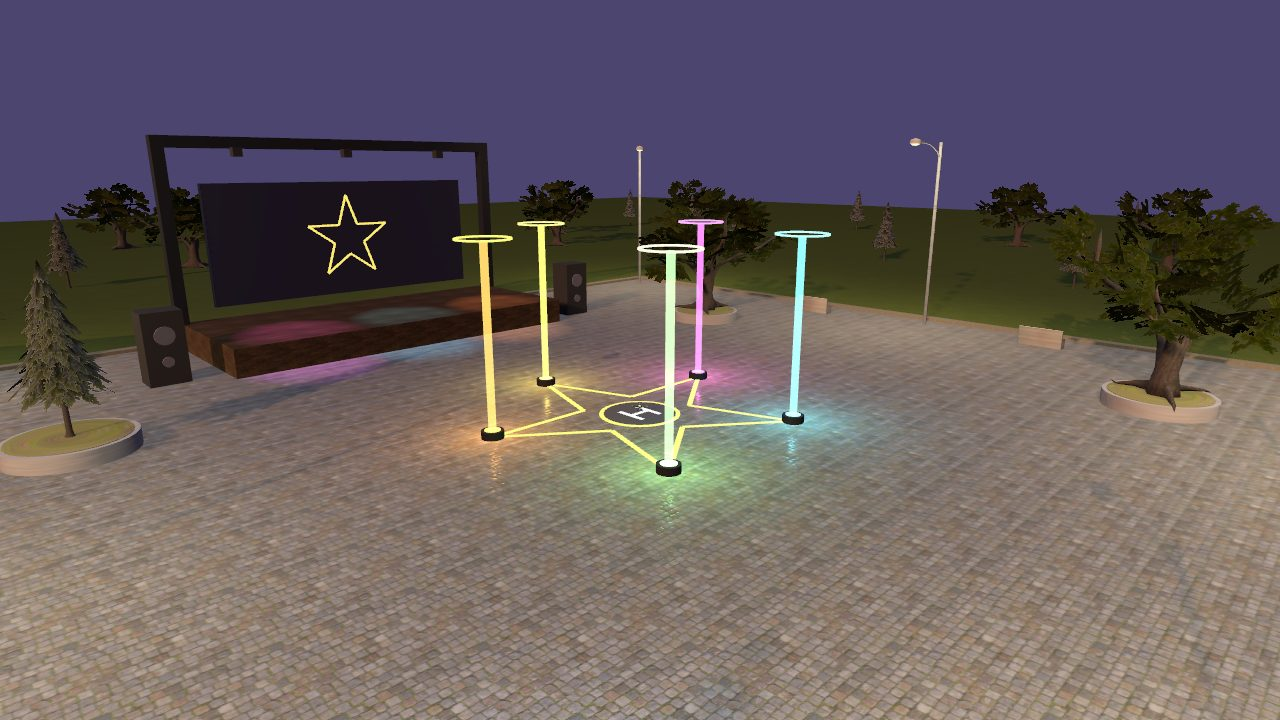
\includegraphics[width=\linewidth]{plaza_show_estrella}};
      \node[anchor=north west,fill=azul,text=white,font=\bfseries\scriptsize,rounded corners=2pt]
        at ([xshift=4pt,yshift=-4pt]im.north west) {MISIÓN 1 · NIVEL 1 \nivel{1}};
    \end{tikzpicture}\\[0.3em]
    \small\textbf{Escenario}: una empresa de espectáculos quiere una \textbf{estrella de 5 picos a 6 m} para el
    show de año nuevo. En cada pico hay una baliza con un \textbf{aro}: el dron pasa por adentro.
    \column{0.41\textwidth}
    \ficha{x500_volando}{x500}{plaza\_show}{estrella\_show}{\cmd{square\_mission}}%
      {los waypoints se \textbf{calculan con una fórmula}}{a \textless 0.5 m de cada vértice}
  \end{columns}
\end{frame}

\begin{frame}{La estrella, paso a paso}
  \begin{columns}[c]
    \column{0.47\textwidth}\centering
    \begin{tikzpicture}[scale=0.55]
      \draw[gray!20,step=1] (-6,-5.6) grid (6,6);
      \draw[-{Stealth},verde,thick] (0,-5.6) -- (0,6.3) node[above,font=\tiny] {N};
      \draw[-{Stealth},rojo,thick] (-6,0) -- (6.3,0) node[right,font=\tiny] {E};
      % las balizas con su aro, en los picos
      \foreach \k in {0,...,4} \draw[naranja,line width=1.2pt] ({5*sin(72*\k)},{5*cos(72*\k)}) circle (0.45);
      % lo recorrido
      \draw[azul,line width=1.8pt,visible on=<4->] (0,5) -- ({1.91*sin(36)},{1.91*cos(36)}) -- ({5*sin(72)},{5*cos(72)})
        -- ({1.91*sin(108)},{1.91*cos(108)}) -- ({5*sin(144)},{5*cos(144)});
      \draw[azul,line width=1.8pt,visible on=<5->] ({5*sin(144)},{5*cos(144)}) -- ({1.91*sin(180)},{1.91*cos(180)})
        -- ({5*sin(216)},{5*cos(216)}) -- ({1.91*sin(252)},{1.91*cos(252)}) -- ({5*sin(288)},{5*cos(288)})
        -- ({1.91*sin(324)},{1.91*cos(324)}) -- (0,5);
      \draw[azul,dashed,thick,-{Stealth},visible on=<3>] (0,0.6) -- (0,4.4);
      \draw[azul,dashed,thick,-{Stealth},visible on=<6>] (0,4.4) -- (0,0.6);
      % el dron
      \only<1-2,6-7>{\node at (0,0) {\dronarriba{1.1cm}};}
      \only<3>{\node at (0,5) {\dronarriba{1.1cm}};}
      \only<4>{\node at ({5*sin(144)},{5*cos(144)}) {\dronarriba{1.1cm}};}
      \only<5>{\node at (0,5) {\dronarriba{1.1cm}};}
    \end{tikzpicture}
    \column{0.52\textwidth}
    \estados{1/WARMUP,2/TAKEOFF,3-5/STAR,6/CENTER,7/LANDING}
    \vspace{0.3em}

    \only<1>{\begin{terminal}{ros2 run x500\_retos estrella\_show}
estrella\_show: 5 picos, radio 5.0 m, a 6.0 m de altura
    \end{terminal}\small En el despegue, que es el \textbf{centro} de la estrella. Calienta setpoints y pide
      Offboard.}%
    \only<2>{\begin{terminal}{estrella\_show}
OFFBOARD activo, subiendo a 6.0 m
    \end{terminal}\small Sube derecho hasta la altura de los aros.}%
    \only<3>{\begin{terminal}{estrella\_show}
En el centro. La figura tiene 11 vértices\\
Vértice 1/11 (0.12 m)
    \end{terminal}\small Llama a \textbf{tu} \cmd{vertices()} y va al primero: el pico \textbf{norte}. Cuenta
      un vértice cuando pasa a menos de 0.5 m y se queda quieto medio segundo.}%
    \only<4>{\begin{terminal}{estrella\_show}
Vértice 5/11 (0.09 m)
    \end{terminal}\small Pico, interior, pico, interior\ldots{} en el orden que regresaste. Cada pico pasa
      por un aro.}%
    \only<5>{\begin{terminal}{estrella\_show}
Vértice 11/11 (0.07 m)\\
Figura completa, regresando al centro
    \end{terminal}\small El vértice 11 es otra vez el pico norte: \textbf{la figura se cierra}.}%
    \only<6>{\begin{terminal}{estrella\_show}
Aterrizando
    \end{terminal}\small De vuelta al centro y aterriza.}%
    \only<7>{\begin{terminal}{estrella\_show}
Aterrizado. Qué tan cerca pasó de cada vértice:\\
\ \ \ 1: 0.12 m OK \ \ldots \ 11: 0.07 m OK\\
Misión cumplida
    \end{terminal}\small El nodo se califica solo: un \textcolor{rojo}{FALLÓ} dice qué vértice está mal
      calculado.}%
  \end{columns}
\end{frame}
